%&latex
%
\providecommand{\main}{../..}
\documentclass[../../main.tex]{subfiles}

\begin{document}

%TODO Missing first part: probably the guided exercise at the end of chapter 11
\section{The Voter Model}
\lesson{33}{25/05/20}

The \textbf{voter model} was originally created in 1975 by Richard A. Holley and Thomas M. Liggett to describe the evolution of people's opinions on polytical parties as consequence of peer pressure.

\medskip

In its most basic form,\marginpar{Basic voter model} each \q{voter} may choose between two possibilities $0$ or $1$, and their beliefs are influenced by their neighbours - meaning that someone voting $1$ that happens to be amongst a group where everyone votes $0$ is likely to change opinion after some time, simply because they hear a lot about $0$.

\medskip

The voter model can be generalized to describe a ecosystem\marginpar{Voter model for ecosystems} with $S$ \textbf{species} (the parties), where each \textbf{node} (person) belongs to one of them, and sits at a position in a $d$ dimensional lattice. Then a \q{person changing ideas} corresponds to a individual of a certain species \textit{dying} and being replaced by a new organism of the neighbouring species - or eventually with an individual of an entirely new species.  

\medskip

To simplify things,\marginpar{Spin-like \textbf{States}} let's focus on only one specific species $A$. Then we define the state $\sigma_x$ of node $x$ as a spin-like variable:
\begin{align*}
    \sigma_x = \begin{cases}
        +1 & \text{if node $x$ is occupied by species $A$}\\
        -1 & \text{otherwise}
    \end{cases}
\end{align*}

At each timestep $n$ \marginpar{\textbf{Dynamics}} a random node $x$ is selected, and the value of $\sigma_x$ is replaced by $\sigma_y$, where $y$ is a randomly chosen \textbf{nearest neighbour} (n.n.) of $x$ \hbox{($y \in \langle x,y \rangle$)}. 

\medskip

Let $w_x(\bm{\sigma})$ be the probability per unit time (i.e. the rate) that spin $\sigma_x$ in state $\bm{\sigma}$ is flipped, i.e. that the transition $\sigma_x \to -\sigma_x$ occurs (leaving all other spins unchanged). 

If all the neighbours of $x$ are equal to $-\sigma_x$, then the transition rate is maximum, and we fix it as $w_x(\bm{\sigma}) \overset{!}{=} 2w$, where $w$ is proportional to the system's \q{reaction speed}, i.e. the reciprocal of its characteristic time $\tau_c$. Conversely, if all neighbours of $x$ are in the same state $\sigma_x$, then no flip will ever occur: $w_x(\bm{\sigma}) = 0$. 

For all the in-between cases, we use a linear interpolation, making the spin-flip rate proportional to the fraction of neighbours of $x$ that \textit{disagree} with $\sigma_x$. Since each node in a $d$-dimensional cubic lattice has $2d$ neighbours, we arrive to the following expression for $w_x(\bm{\sigma})$:
\begin{align}\label{eqn:spin-change1}
    w_x(\bm{\sigma}) = \left[1- \frac{1}{2d}(n_{\sigma_x} - n_{-\sigma_x}) \right] w = \frac{n_{-\sigma_x}}{d} w 
\end{align}
where $n_{\pm \sigma_x}$ is the number of n.n. of $x$ with state $\pm \sigma_x$.

Note that if $\sigma_y = \sigma_x$, then $\sigma_y \sigma_x = +1$, and otherwise we have $\sigma_y \sigma_x = -1$. So:
\begin{align*}
    n_{\pm \sigma_x} = \pm \sum_{\mathclap{y \in \langle x,y \rangle}} \sigma_x \sigma_y
\end{align*}
And substituting back in (\ref{eqn:spin-change1}) leads to:
\begin{align}\label{eqn:spin-change2}
    w_x(\bm{\sigma}) = \left[1 - \frac{1}{2d} \sigma_x \sum_{\mathclap{y \in \langle x,y \rangle}} \sigma_y \right] \cdot w
\end{align}
Then, similarly to what we did in sec. \ref{sec:dynamics-ising}, the transition rate from state $\bm{\sigma'}$ to any other state $\bm{\sigma}$ can be written as the sum over the necessary spin-flip transitions:
\begin{align*}
    W(\bm{\sigma}|\bm{\sigma'}) = \sum_x w_x(\sigma) \delta_{\sigma_x, -\sigma_x'}\Big[ \prod_{z \neq x} \delta_{\sigma_z', \sigma_z} \Big]
\end{align*}

\begin{figure}[H]
    \centering
    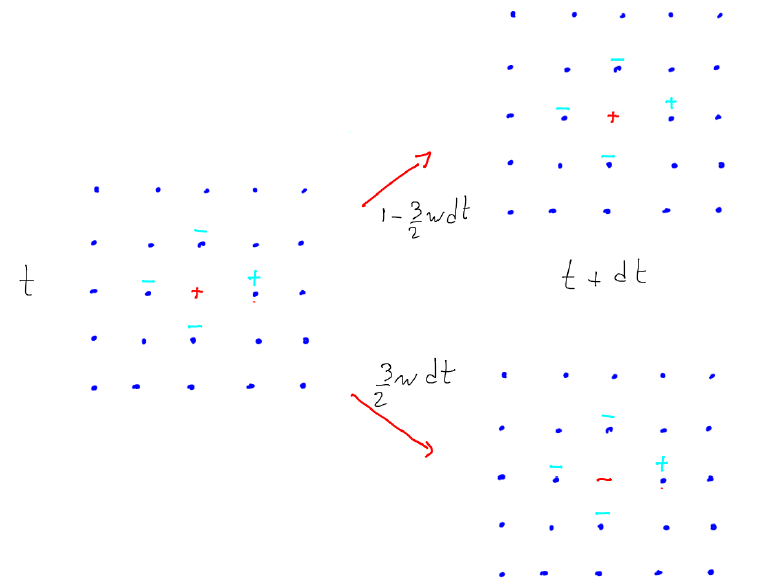
\includegraphics[width=0.8\textwidth]{spin-flips.png}
    \caption{Example of spin-flip transitions on a $d=2$ lattice. The red $\textcolor{Red}{+1}$ spin has $1$ neighbour \textit{agreeing} with it ($n_{+1} = 1$) and $3$ that \textit{disagree} with it ($n_{-1} = 3$). The maximum possible flip rate is $2w$, but since only $3/4$ of neighbours disagree, the final rate will be $3w/2$, leading to a transition \textbf{probability} of $3w \dd{t}/2$. Conversely, the transition probabilities with \textit{no spin-flip} will be $1-3w\dd{t}/2$.}
    \label{fig:spin-flips}
\end{figure}

Let $\bm{\sigma}$ be a spin configuration, and denote with $\bm{\sigma^{(x)}}$ the configuration resulting from flipping \textit{only} spin $x$ of $\bm{\sigma}$, i.e. such that:
\begin{align*}
    \sigma_x^{(x)} = -\sigma_x; \qquad \sigma_y^{(x)} = \sigma_y \quad \forall y \neq x
\end{align*} 
We can then write the system's Master Equation:\marginpar{\vspace{2em}Master Equation}
\begin{align}\label{eqn:voting-ME}
    \dot{P}(\bm{\sigma};t) = \sum_x [\underbrace{w_x(\bm{\sigma^{(x)}}) \mathbb{P}(\bm{\sigma^{(x)}}; t)}_{\text{\q{Inward} flux}}  - \underbrace{w_x(\bm{\sigma}) \mathbb{P}(\bm{\sigma}; t)}_{\text{\q{Outward} flux}} ]
\end{align}

% Two key questions:
% \begin{enumerate}
%     \item What is the probability that a certain species will persist forever?
%     \item In which conditions can many species coexist?
% \end{enumerate}

\subsection{Correlation functions}
In order to get some insight on the dynamics, we compute the evolution of the $1$ and $2$-point correlation functions.

\subsubsection{1-point correlation}

First, consider the following change of variables, from \textit{spin}-like ($\pm 1$) to \textit{binary} ($\{0,1\}$):
\begin{align}\label{eqn:presence-indicator}
    \frac{1+\sigma_z}{2} = \begin{cases}
        1 & \text{if the chosen species is occupying node $z$}\\
        0 & \text{otherwise}
    \end{cases} 
\end{align}  
The probability that a given species is present at $x$ at time $t$ is given by averaging the indicator \textit{binary} variable of \q{presence} over all nodes:
\begin{align*}
    \langle \frac{1+ \sigma_z}{2}  \rangle_t = \frac{1+\langle \sigma_z \rangle_t}{2} 
\end{align*}


\end{document}
